\chapter{Conclusion}

The presented approach in this study is effective for symbol recognition with symbols with different levels of noise and geometric transformations. Also this approach, is not only effective for symbol recognition only but for any isolated pattern recognition due to the fact that no prior information about the pattern is used. This makes the presented approach a versatile one which can be used in various other applications. \\

\section{Outlook}
For future work, the next part of this study is to evaluate the effectiveness of the approach used so far on the last set of datasets. The fourth category of datasets consists of three different datasets called Set A, Set B and Set C which have 50, 100 and 150 different models respectively. These model symbols consist of both straight lines and arcs or circles.  All datasets contain 50 test images per model symbol. Therefore the number of total test images per dataset varies where Set A contains 2500 testing images, Set B contains 5000 testing images and Set C contains 7500 test images. Scaling and orientation vary from those in the model through out each of the test symbols. Noise is introduced in the form of added noise or line thickening or line degradation. These types of noises are never applied together Fig. \ref{fig:SetCExamples} illustrates a few samples.\\
 
\begin{figure*}[h]
        \centering
                \begin{subfigure}[b]{0.2\textwidth}
                \centering
                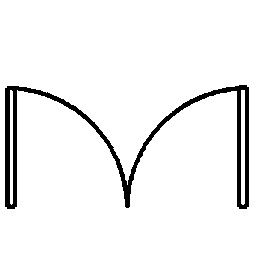
\includegraphics[width=1.1\textwidth]{figures/Results/SetC/Model.png}
                \caption{}
        \end{subfigure}\\
                \begin{subfigure}[b]{0.25\textwidth}
                \centering
                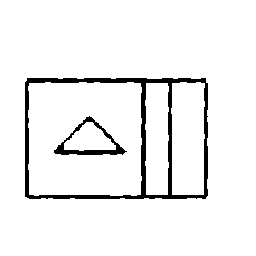
\includegraphics[width=0.9\textwidth]{figures/Results/SetC/1.png}
                \put(8,40){$\cdots$}
                \caption{}
        \end{subfigure}
        \qquad
                \begin{subfigure}[b]{0.25\textwidth}
                \centering
                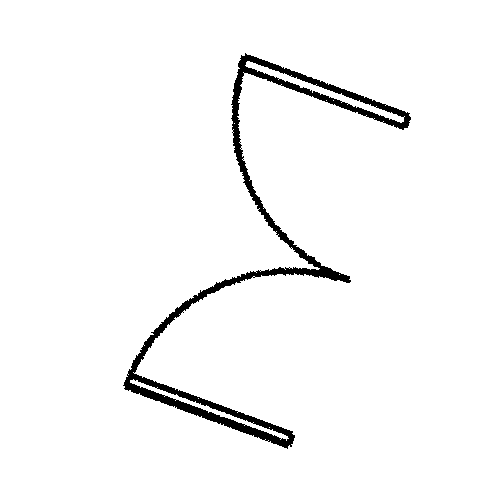
\includegraphics[width=0.9\textwidth]{figures/Results/SetC/2.png}
                \put(8,40){$\cdots$}
                \caption{}
        \end{subfigure}
        \qquad
                \begin{subfigure}[b]{0.25\textwidth}
                \centering
                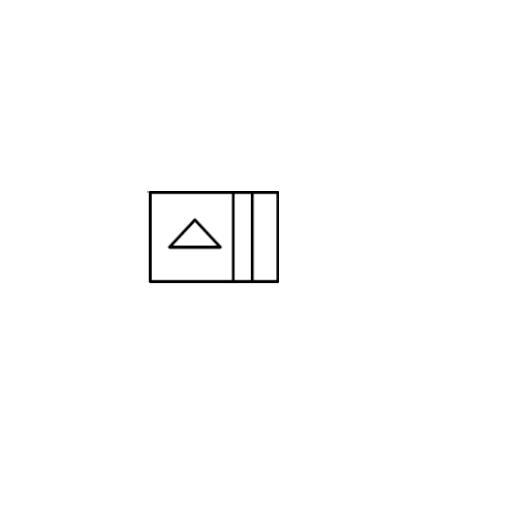
\includegraphics[width=0.9\textwidth]{figures/Results/SetC/3.png}
                \caption{}
        \end{subfigure}
        \caption[Sample data from the 'Set C' dataset]{(b) (c) (d) Three test images for (a) a model symbol are illustrated from the Set C dataset }
        \label{fig:SetCExamples} 
\end{figure*}        

The final results during the GREC'11 contest, associated with these datasets, are shown in the following table \cite{Delalandre_2012}.

\begin{table}[h]
\centering
\caption{Contest's global results. Adapted from \cite{Delalandre_2012}}
\begin{tabular}{ccccccccccccccc}
  \hline
      Test Name & & & & & & & & Recognition Rate \\
  \hline
      set 1 (50 models) & & & & & & & &  94.76 \% \\
      set 2 (100 models) & & & & & & & &  91.98 \% \\
      set 3 (150 models) & & & & & & & &  85.88 \% \\

  \hline
\end{tabular}
\end{table}


In this study, the experiments were implemented using a MATLAB environment. Furthermore, the experiment code was developed using a sequential approach. Future work on this regard may include the re-writing of experiments by adhering to a parallel model using different more efficient languages such as C++. This will help improve time effeciency in which COSFIRE operators are configured and applied, and the time in which test images are classified. \\

An interesting work would also be to evaluate experimental results using different values for a number of COSFIRE parameters such as alpha and sigma0. These two parameters control the tolerance of the mutual spatial arrangement of the involved contour parts.\\

A different approach can also be taken towards which classification methods to use. In this study a KNN algorithm was used to classify the test images. The distance metric used in the KNN algorithm was Euclidean. Different distance metrics can be implemented and investigated for classification. Also apart from the KNN algorithm, other classification techniques that can be considered. \\

Also, this approach's robustness and scalability to noise or transformations can be investigated against different types of symbol datasets such as characters, musical symbols, etc. Also for datasets which are comprised of more than one image per model, different classification methods such as artificial neural networks, graphs, support vector machines, can be used. \\




